

\newpage
\begin{center}
    \textbf{\large 4. FLUTTER ПРИЛОЖЕНИЕ}
\end{center}
\refstepcounter{chapter}
\addcontentsline{toc}{chapter}{4. FLUTTER ПРИЛОЖЕНИЕ}

Мобильное приложение для получения расписания МТУСИ создано на базе фреймворка Flutter 
и предназначено для студентов, преподавателей и сотрудников университета. 
Пользователи могут выбрать свою группу, аудиторию, преподавателя, предмет и даты, 
на которые они хотят получить расписание занятий и экзаменов. 
После выбора фильтров, приложение обращается к GraphQL API, чтобы получить данные о занятиях и экзаменах, 
соответствующих заданным фильтрам.

Приложение имеет удобный интерфейс, который позволяет просматривать расписание. 
Кроме того, приложение позволяет экспортировать расписание в формате ICS, и добавлять в календарь.
Для удобства использования приложение имеет функции быстрого поиска и фильтрации,
которые позволяют пользователям быстро находить нужную информацию.
Кроме того, приложение сохраняет последний запрос в кеше устройства,
чтобы пользователи могли быстро вернуться к предыдущим поискам.

Мобильное приложение для получения расписания МТУСИ является удобным и
эффективным инструментом для студентов, преподавателей и сотрудников университета,
которые хотят быть в курсе своего расписания занятий и экзаменов.

\section{Обзор технологий, использованных при разработке приложения}

\textbf{Flutter} --- это фреймворк для разработки мобильных приложений,
созданный компанией Google.
Он позволяет создавать высокопроизводительные приложения для Android и iOS
с использованием одного и того же кода на языке программирования Dart.
Flutter использует собственный движок для отрисовки пользовательского интерфейса,
что позволяет достичь высокой производительности и кроссплатформенной совместимости.
Flutter также предоставляет широкий набор виджетов и инструментов для создания красивого
и интуитивно понятного пользовательского интерфейса.

\textbf{Реактивный подход} --- это подход к разработке программного обеспечения,
который основан на обработке изменений данных. 
В реактивном подходе данные представляются в виде потоков,
которые изменяются во времени.
При изменении данных в потоке, происходит обновление пользовательского интерфейса.

\textbf{PWA (Progressive Web Application)} --- это веб-приложение, 
которое можно использовать как обычное приложение на мобильных устройствах 
и настольных компьютерах. PWA обладает некоторыми преимуществами 
перед обычными веб-приложениями, такими как возможность работы без 
подключения к Интернету, быстродействие и возможность установки 
на домашний экран мобильного устройства. PWA также имеет 
возможность использования нативных функций устройства, 
таких как уведомления и доступ к камере, что делает его 
более удобным и функциональным для пользователей.

\section{Функции приложения}
\subsection{Экран поиска}
Экран поиска является одной из ключевых функций сервиса.
Он позволяет пользователям быстро находить расписания занятий и экзаменов по различным параметрам.

Пользователи могут искать информацию по:
\begin{itemize}
    \item Группе
    \item Аудитории
    \item Преподавателю
    \item Предмету
\end{itemize}

Подсказки отображаются на экране поиска в реальном времени, когда пользователь начинает вводить запрос.
Когда пользователь начинает вводить буквы, экран поиска предлагает список наиболее подходящих результатов,
основанных на уже введенных символах.
Например, если пользователь начинает вводить название группы,
экран поиска предлагает список всех групп, у которых в названии есть введенные символы.
Пользователь может выбрать нужную группу из списка и получить соответствующее расписание занятий и экзаменов.
Этот механизм упрощает и ускоряет поиск информации для пользователей,
делая сервис более удобным и эффективным.

На экране поиска есть кнопка "Добавить в календарь",
которая позволяет пользователям подписаться на календарь по URL
и получать обновленное расписание занятий и экзаменов
в своем календаре без необходимости ручного импорта файла.
Это реализовано при помощи микросервиса, который генерирует ICS-файл
на основе полученных данных и сохраняет его в файловое распределенное хранилище S3.
При последующих обращениях по URL микросервис проверяет актуальность
уже генерированного файла при помощи механизма ведения ревизий,
и если файл все еще актуальный - возвращает HTTP код переадресации на ICS из файлового хранилища.

\begin{figure}[h]
\centering
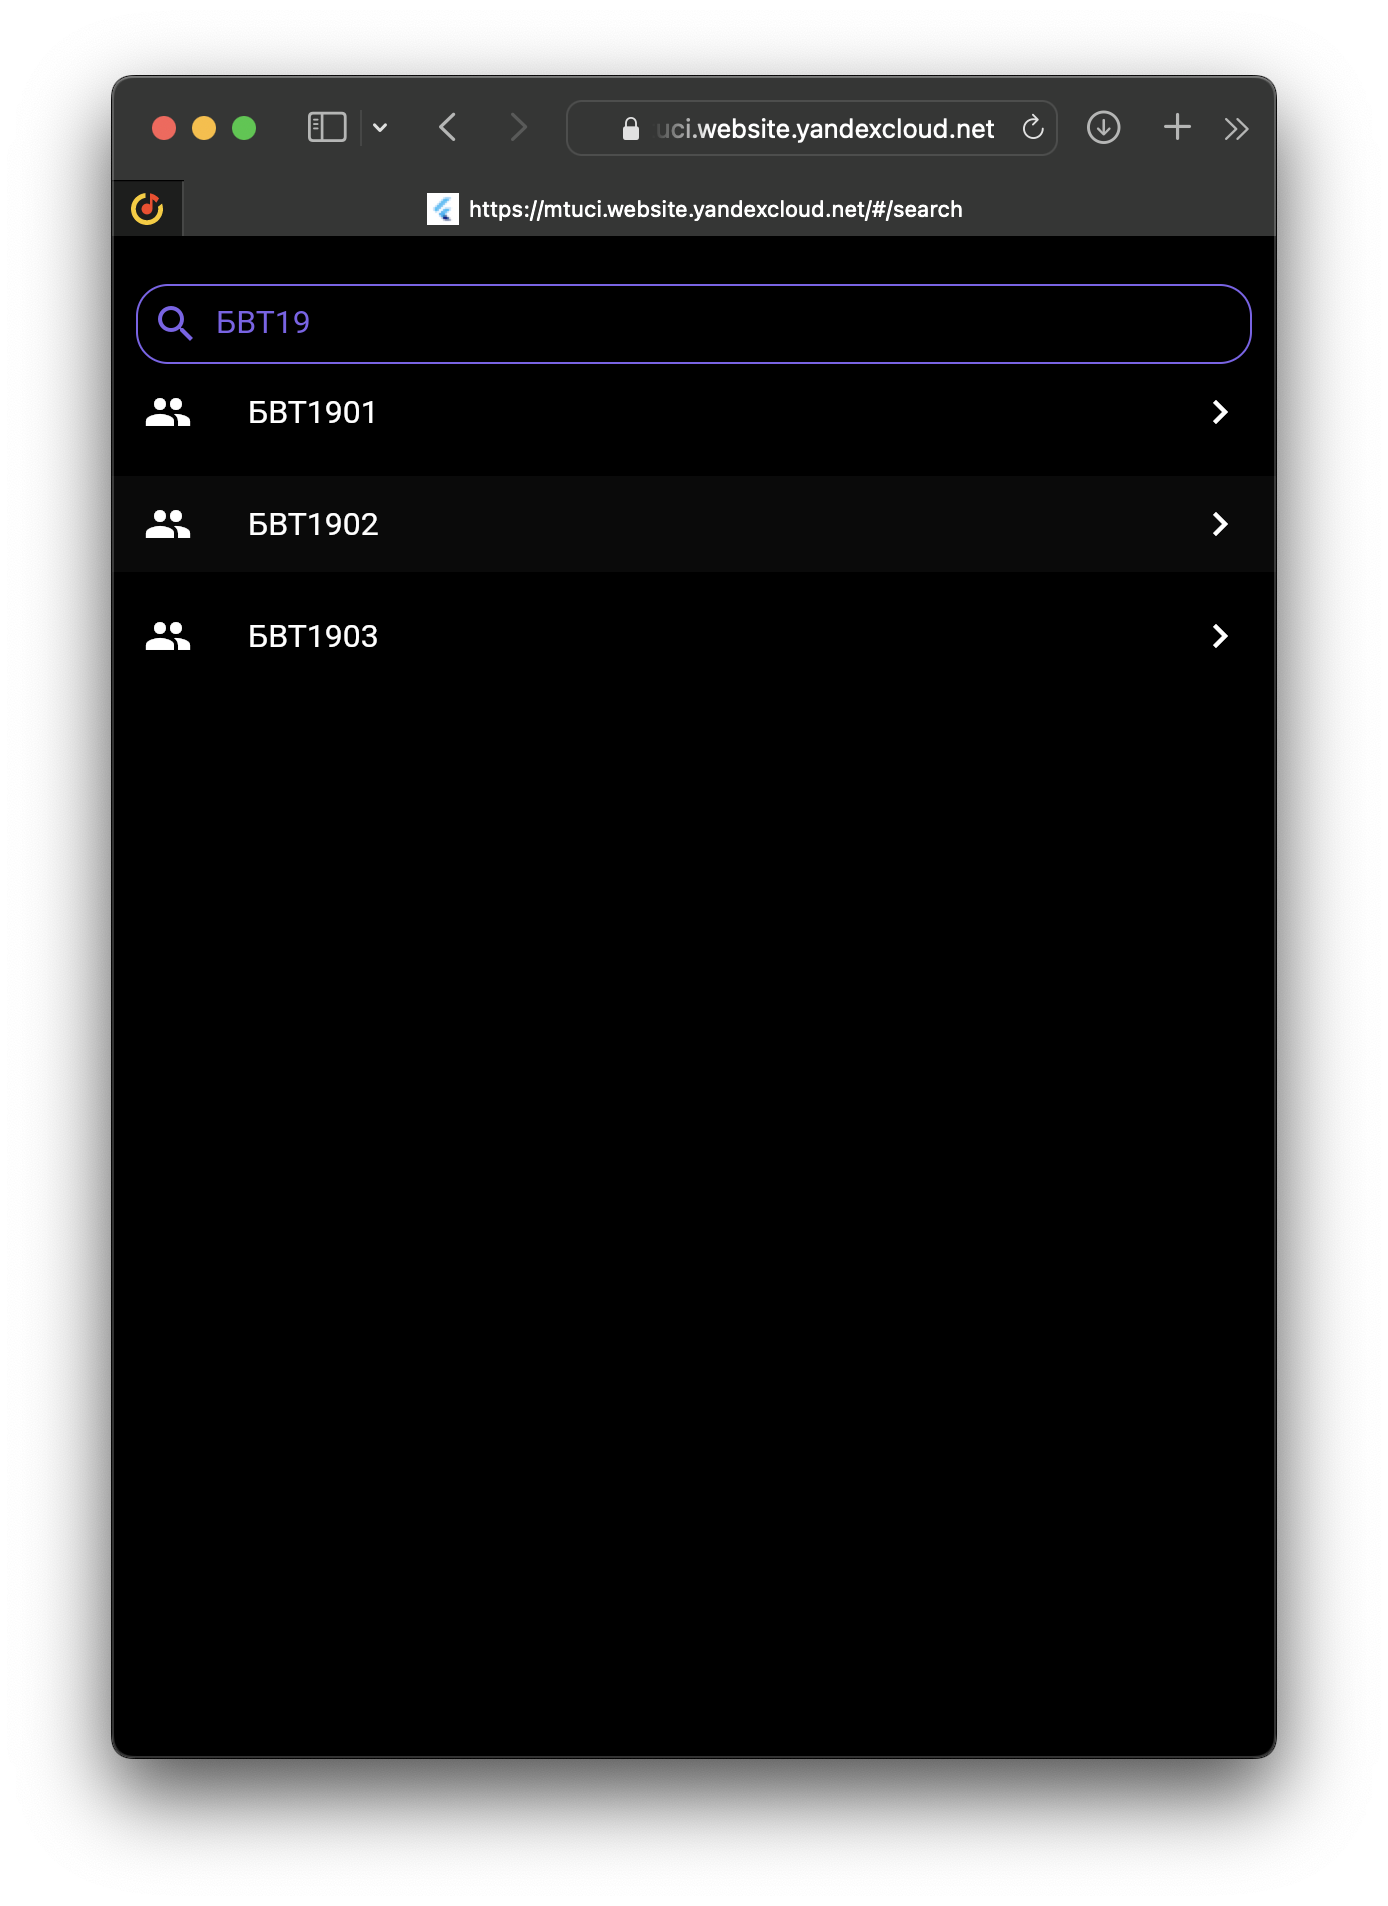
\includegraphics[width=0.8\linewidth]{images/search_screen.png}
\caption{Скриншот экрана поиска}
\label{fig:mpr}
\end{figure}

\subsection{Экран расписания}
Экран расписания является одним из ключевых элементов приложения для получения расписания МТУСИ.
На этом экране пользователи могут увидеть расписание занятий на конкретный день.

Экран содержит следующие элементы:

\begin{itemize}
    \item Возможность возврата к поиску, 
    чтобы пользователи могли быстро изменить параметры поиска и найти нужное расписание.
    \item Расписание занятий на конкретный день.
    Пользователи могут просмотреть расписание занятий для выбранной группы,
    преподавателя, аудитории или предмета на любую дату.
    \item Если на выбранный день нет занятий,
    то есть кнопка, которая ведет к ближайшим датам занятий.
    Пользователи могут увидеть, когда будут следующие занятия и планировать свое время соответственно.
\end{itemize}


\begin{figure}[h]
\centering
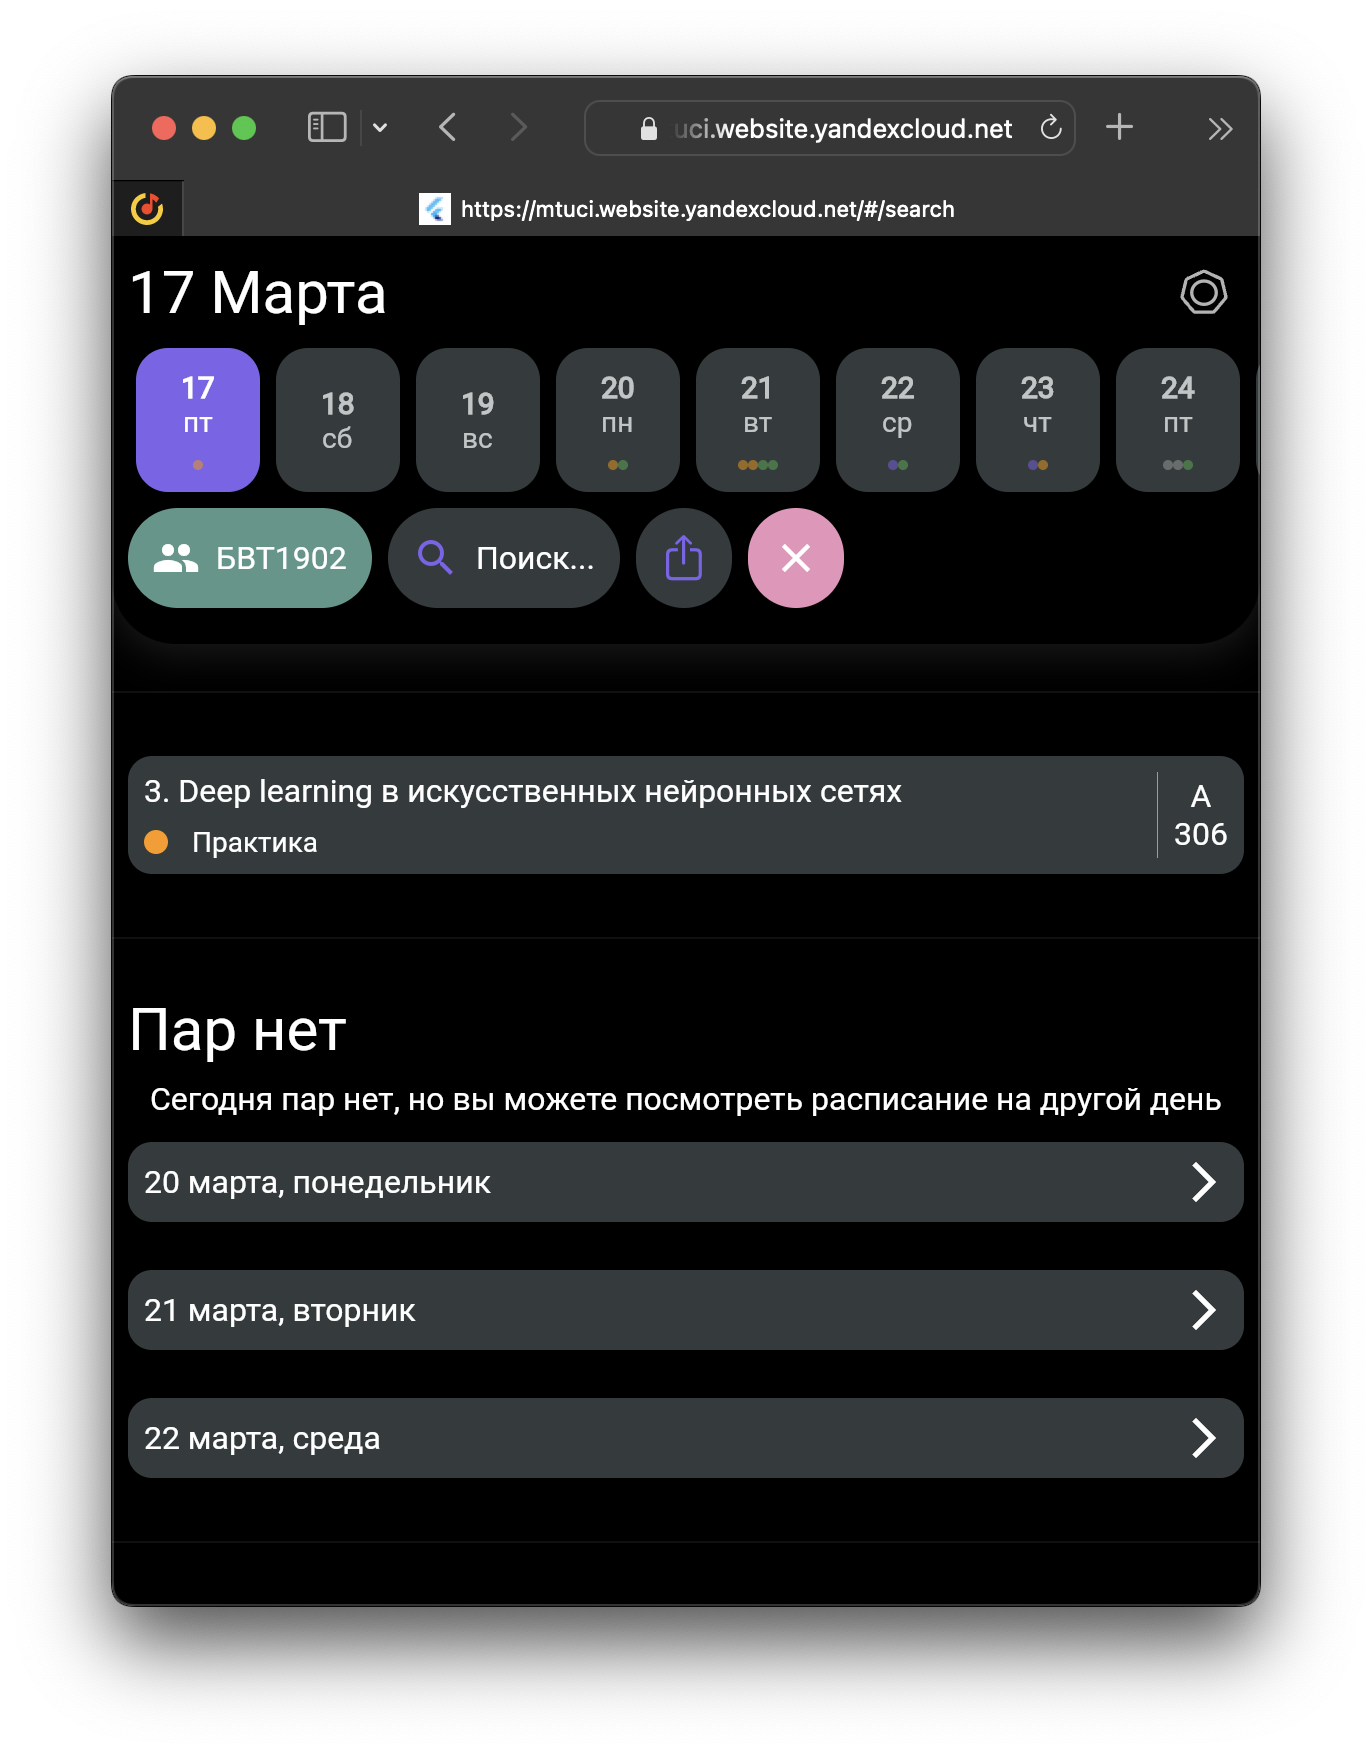
\includegraphics[width=0.8\linewidth]{images/rasp_screen.png}
\caption{Скриншот экрана расписания}
\label{fig:mpr}
\end{figure}

В целом, экран расписания является важным элементом приложения
для получения расписания МТУСИ, который помогает пользователям оставаться
в курсе своих занятий и экзаменов.

\subsection{Экран настроек}
Экран настроек предоставляет пользователям возможность настроить
приложение на свой вкус и свои потребности.
Он содержит ряд настроек, которые помогают улучшить
пользовательский опыт и сделать использование приложения более комфортным.

В приложении можно регулировать следующие настройки:
\begin{itemize}
    \item Настройка \textbf{языка} приложения позволяет пользователям лучше понимать интерфейс и функциональность приложения.
    \item Экран настроек также позволяет выбрать \textbf{тему} приложения (темную или светлую),
    которая наиболее комфортна для глаз и соответствует условиям окружающей среды. 
    \item Наконец, пользователи могут отправить \textbf{сообщение разработчику} приложения,
    чтобы получить поддержку в случае необходимости.
\end{itemize}

\begin{figure}[h]
\centering
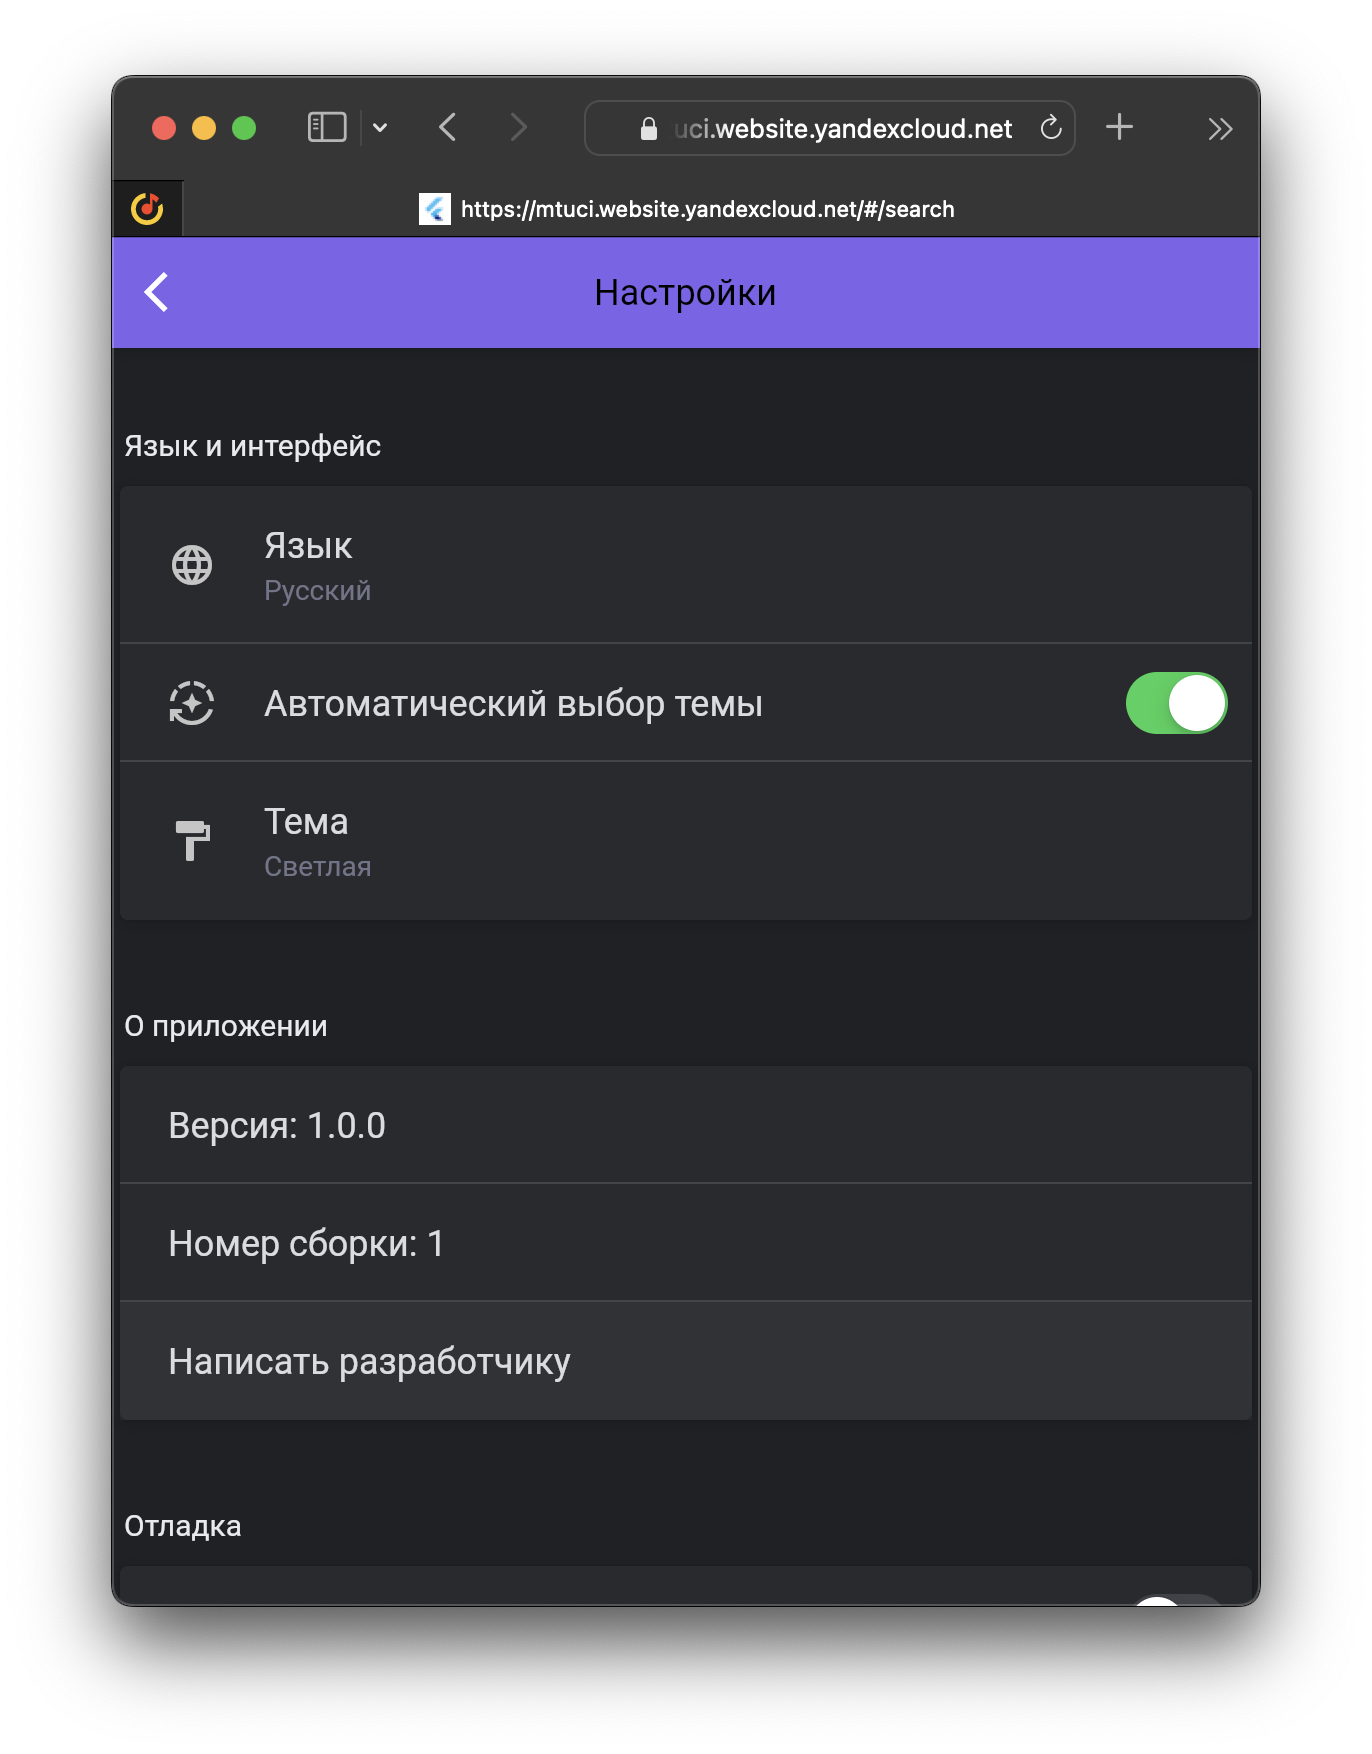
\includegraphics[width=0.8\linewidth]{images/settings_screen.png}
\caption{Скриншот экрана настроек}
\label{fig:mpr}
\end{figure}

В целом, экран настроек является важным элементом приложения,
который помогает пользователям настроить приложение на свой вкус и
решить любые вопросы, связанные с использованием приложения.

\subsection{Экран одного занятия}
На экране одного занятия пользователи могут получить подробную информацию о конкретном занятии или экзамене.
Этот экран предоставляет детали занятия,
такие как:
\begin{itemize}
    \item Дата
    \item Время
    \item Место проведения
    \item Название группы
    \item ФИО преподавателя
    \item Название предмета
\end{itemize}

\begin{figure}[h]
\centering
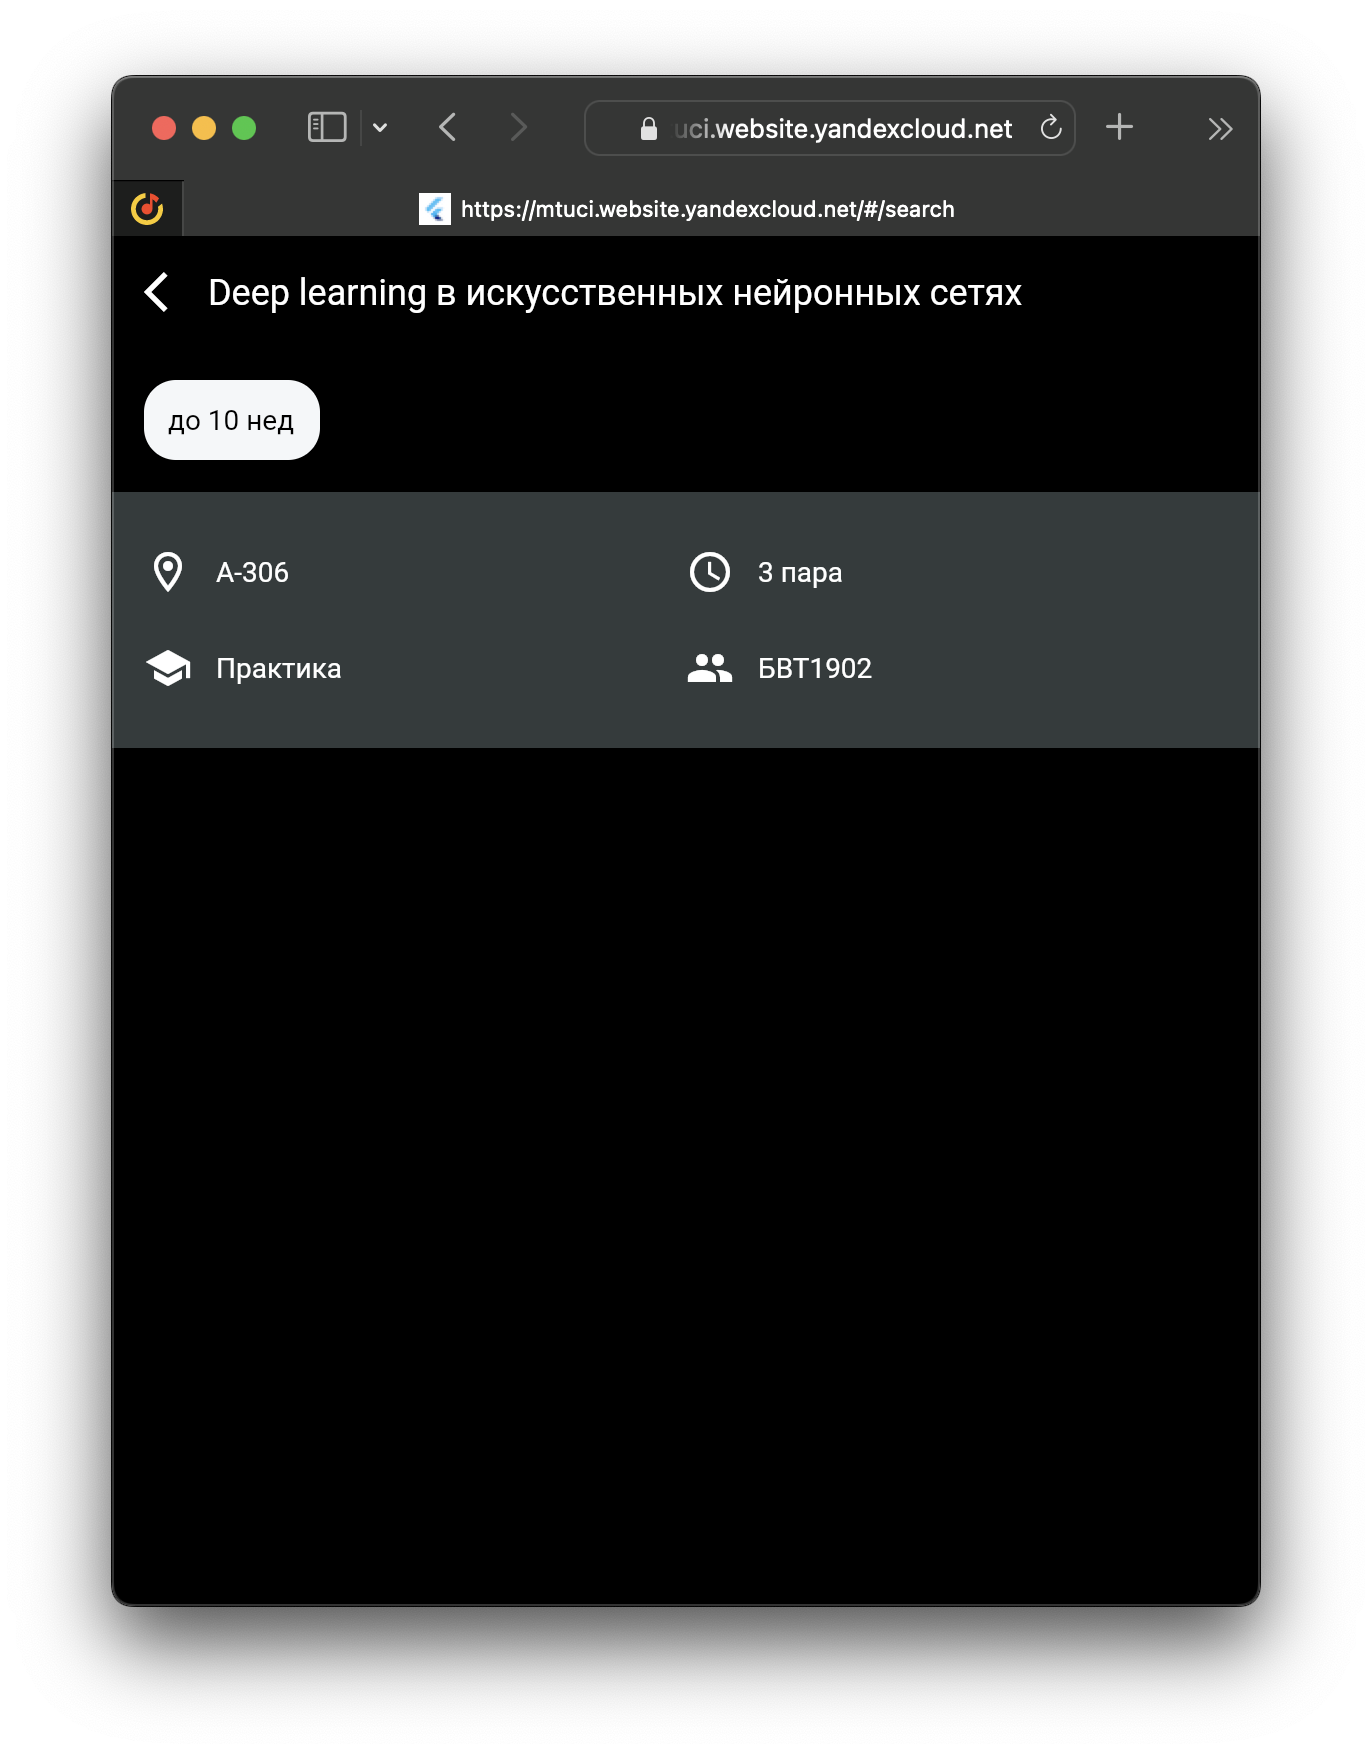
\includegraphics[width=0.8\linewidth]{images/lesson_screen.png}
\caption{Скриншот экрана одного занятия}
\label{fig:mpr}
\end{figure}

Экран одного занятия является важным элементом приложения,
который помогает пользователям получать детальную информацию
о своих занятиях и планировать свое расписание соответственно.
Благодаря этому экрану, пользователи могут легко организовать
свое время и не пропускать важные занятия и экзамены.

\section{Кроссплатформенность}
Приложение разрабатывается с учетом кроссплатформенности и может быть запущено на различных платформах,
включая iOS, Android и веб-браузеры.
Для этого используются современные технологии разработки, такие как Flutter и GraphQL API.
Такой подход позволяет достичь максимальной доступности приложения для пользователей и обеспечить единый
интерфейс и функциональность на разных платформах.

\begin{itemize}
    \item \textbf{WEB} - приложение доступно в браузерах, таких как Google Chrome, Mozilla Firefox и Safari. 
    Оно адаптировано для работы на смартфонах, и может быть добавлено на главный экран как PWA (Progressive Web App).
    На данный момент приложение доступно по адресу \url{https://mtuci.website.yandexcloud.net}.
    \item \textbf{Android} - приложение доступно для смартфонов и планшетов на базе операционной системы Android.
    На данный момент приложение можно загрузить по адресу \url{https://storage.yandexcloud.net/mtuci/app-release.apk}.
    \item \textbf{iOS} - приложение доступно для смартфонов и планшетов на базе операционной системы iOS.
\end{itemize}

\section{Интеграция с GraphQL API}
Приложение использует GraphQL API для получения данных о расписании занятий и экзаменов. 
GraphQL API предоставляет единый интерфейс для доступа к данным из различных источников, 
включая базу данных, внешние API и другие источники данных. 
Это позволяет приложению получать данные быстро и эффективно, 
а также обеспечивает возможность масштабирования приложения при необходимости. 
Кроме того, GraphQL API позволяет запросить только необходимые данные, 
что уменьшает нагрузку на сеть и повышает производительность приложения.

Кеширование данных является важным элементом производительности и оптимизации приложения. 
В приложении используется механизм кеширования данных на стороне клиента, 
который позволяет уменьшить количество запросов к серверу и ускорить загрузку данных.
